\documentclass[../primer.tex]{subfiles}

\begin{document}

\chapter{Exploration}

\section{Sensitivity Analysis}
\subsection{Motivation} \label{sec:orgdc914a7}
Here at Stanford,\footnote{Circa 2018} we host the Predictive Science Academic
Alliance Program II
(\href{http://exascale.stanford.edu/content/stanford-psaap-ii-motivation-1}{PSAAP
  II}). This project is motivated by a solar receiver intended for green energy
production, with heat transfer enhanced via a particle-laden working fluid. This
is a system of enormous complexity, featuring particle-laden turbulent flow with
radiative heat transfer. The difficulty arises (in part) due to the complex
multiphysics, which necessitates careful modeling for computational
tractability. For example, the Stanford PSAAP II simulation codes implement
models not just for the turbulence, but also novel models for radiation
transport, accounting for distributed particles smaller than the resolved
gridsize.

\begin{figure}[!ht]
  \centering
  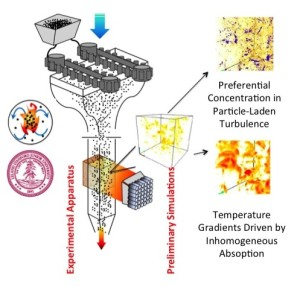
\includegraphics[width=0.75\textwidth]{./images/psaap}
  \caption{Schematic for the PSAAP II physical problem. This graphic
    highlights some of the complex interactions between traditionally
    separate domain physics. The complexity of the physics necessitates
    modeling assumptions, which introduce uncertainties.}
  \label{fig:psaap}
\end{figure}

\marginnote{Note that some of the techniques we will discuss are
sample-intensive. Most of the techniques described below are intended for
\emph{computer experiments}; that is, simulation campaigns run on computer codes.
Contrast these with \emph{physical experiments}, in which the physical
world `solves' the equations of motion automatically.}

\clearpage

These modeling assumptions introduce non-physical coefficients, which constitute
additional uncertainties in the problem. Table \ref{tab:uncertainties} lists
these and other examples of uncertainties in the PSAAP II problem. For practical
purposes, we would be interested in how \emph{all} the uncertainties affect practical
output quantities of interest, such as the device efficiency. If the results
were largely insensitive to our uncertainties over a range of physically
relevant values, this would build confidence in our ability to perform accurate
simulations, and would potentially enable the design of novel solar receivers.

\begin{table}[!ht]
\caption{A non-exhaustive list of examples of uncertainties
in the Stanford PSAAP II problem.}
\label{tab:uncertainties}
\begin{tabular}{@{}ll@{}}
Type                       & Source                        \\
\hline
Input Uncertainties        & Turbulence model parameters   \\
Model Discrepancies        & Limitations of eddy viscosity \\
Numerical Errors           & Artificial dissipation        \\
Experimental Uncertainties & Probe accuracy limitations    \\
\end{tabular}
\end{table}

If our outputs were \emph{not} insensitive to these uncertainties, that would signal
that we need to either reduce the uncertainties (say through experimentation),
or account for the uncertainties in our results (say through uncertainty
propagation). This would necessitate a combination of experimental and
computational work -- both are expensive activities.

This expense is compunded by the \emph{curse of dimensionality}, which states
(roughly) that the expense of a procedure\footnote{e.g. a parameter study, or
numerical quadrature} tends to grow \emph{exponentially} with dimension. Not only is
gathering data expensive; we need many data points to understand
high-dimensional parameter spaces!

\begin{figure}[htbp]
\centering
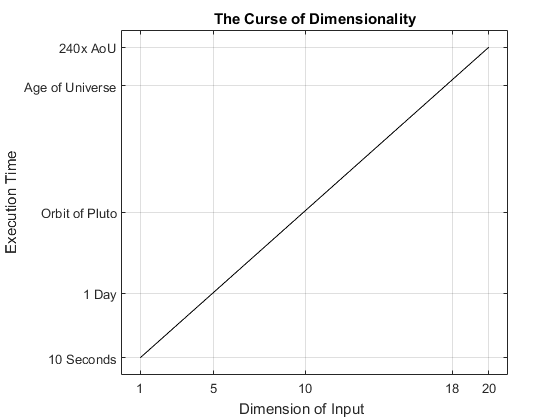
\includegraphics[width=.9\linewidth]{./images/curse_of_dimensionality.png}
\caption{Cartoon depicting computational expense under the curse of dimensionality. Imagine that we are performing quadrature (numerical integration), and are using a simple tensor-product approach; i.e. using 10 evaluations per dimension. If a computer implementation of our qoi evaluates in one second, it will take 10 seconds to study a 1-dimensional function. For a 5-dimensional function, this will take a day to evaluate. This exponential growth quickly grows out of hand, reaching an execution time of nearly the Age of the Universe at just 18 dimensions.}
\end{figure}

Ideally, one would like to know which parameters are most influential,
preferably before embarking on an expensive simulation campaign. This is the
insight that sensitivity analysis seeks to provide. A sensible way to address
this curse is to attack dimensionality directly -- to reduce the number of input
parameters. As a simple approach, we could perform a sensitivity analysis,
identify those parameters which do not appreciably affect our qoi, and freeze
them to nominal values. This effectively reduces the dimensionality of the
problem, ameliorating the curse of dimensionality.

An intermediate conclusion

Sensitivity analysis is about determining how input parameters affect a chosen
quantity of interest. We would apply these results at multiple stages in an
analysis. A sensitivity analysis could help identify which uncertainties are
worth characterizing through a physical experiment. Such an analysis could
also identify parameters which can be frozen to nominal values, making further
computational experiments less expensive.

\subsection{Local vs Global}
\label{sec:org4eb0133}
There are two broad philosophies to sensitivity analysis: local and global.
Local sensitivity generally refers to studying the gradient of a qoi; the
derivative (partial or total) of the output qoi with respect to its input
parameters, computed at a set of nominal values. Global sensitivity generally
refers to variance contributions; the amount of variance exhibited in the output
qoi, as contributed by different sets of the input parameters.

\begin{figure}[!ht]
  \centering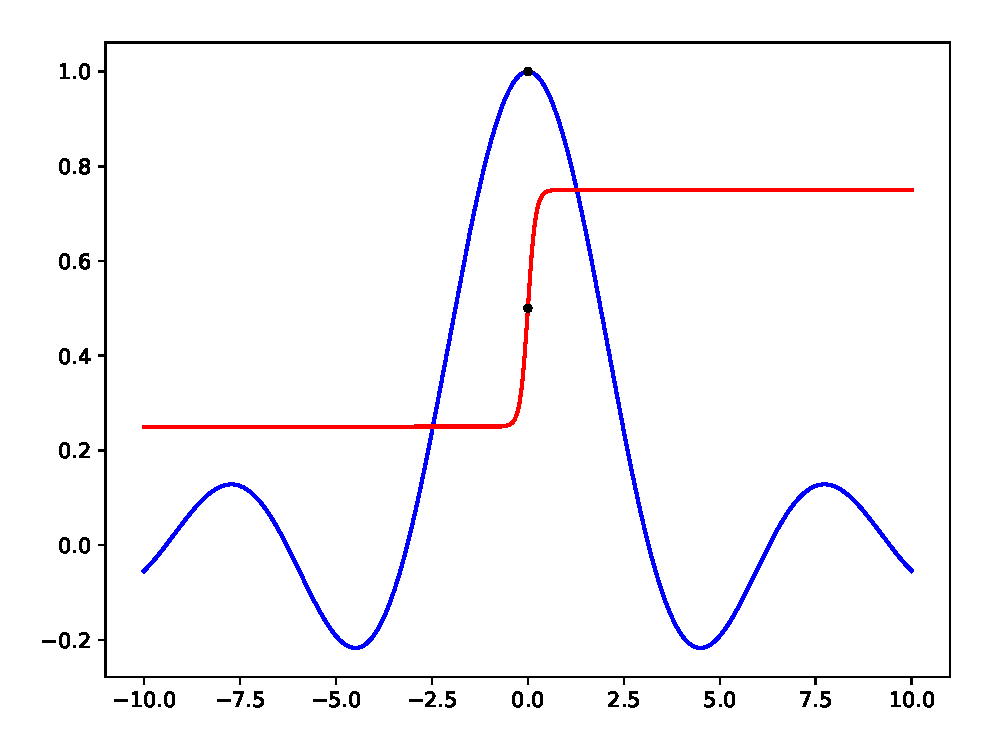
\includegraphics[width=0.75\textwidth]{./images/ex1}
  \caption{Cartoon functions to depict differences between local and global
  sensitivity. The vertical axis corresponds to our qoi, while the horizontal
  corresponds to an input parameter. The black dot is the point of interest
  for local sensitivity. The blue curve has a great deal of global sensitivity,
  but zero local sensitivity. The red curve has comparatively little global
  sensitivity, but a large local sensitivity. Which metric is important
  depends on the objective of the study.}
  \label{fig:ex1}
\end{figure}

As implied by the names, the two approaches give different pieces of
information. Depending on the context, one or the other may be the `right'
metric to study. Figure \ref{fig:ex1} provides a simple cartoon illustration of
two cases where local and global sensitivities will be in disagreement.

In what follows, we will focus on local sensitivity, and leave global
sensitivity to a following set of notes.

\subsection{Preliminary Considerations}
\label{sec:org797e9af}
Before we jump into computing the derivative, we will first discuss some
preliminary concerns. Before computing the derivative, we ought to determine
\emph{where} we ought to evaluate! Furthermore, we ought to have some clear goal in
mind of what to \emph{do} with the gradient before we set out to compute it.

To introduce some notation, let \(f(\vx):\R{d}\to\R{}\) be our quantity of
interest (qoi), and let \(\Omega\subseteq\R{d}\) be the parameter space of
interest. The first object we'll study is \(\Omega\).

Region identification

The parameter space \(\Omega\) may itself be uncertain, or at least poorly
characterized. It is possible that insights gained in one subset of \(\Omega\) may
not hold in other regions, or modeling choices which are appropriate in one
region may fail in another. Figure \ref{fig:moody} depicts a classical example
from fluid mechanics where physical behavior changes dramatically in different
regions of parameter space. The punchline here is that one should think
carefully about the domain \(\Omega\) to be studied, as this will affect the
conclusions drawn from sensitivity analysis, either local or global.

\begin{figure}[!ht]
  \centering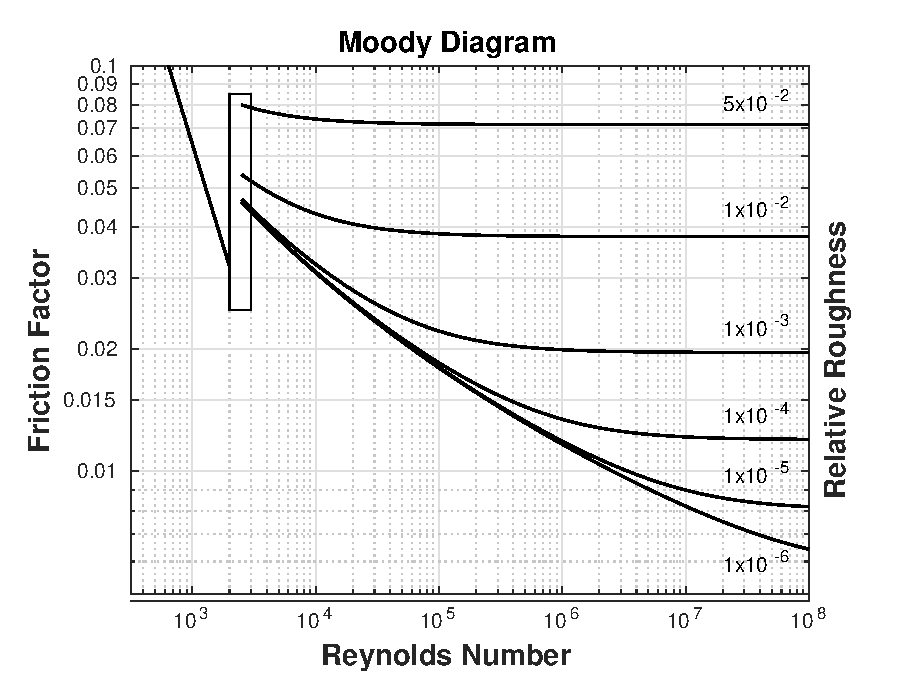
\includegraphics[width=0.75\textwidth]{./images/moody_diagram}
  \caption{The Moody Diagram depicts the dimensionless pressure losses (Friction Factor)
  against relevant dimensionless parameters. Note that the Relative Roughness only
  becomes relevant at high Reynolds Number. This sort of information would not be
  discovered through a global sensitivity analysis, and instead requires careful
  probing of local properties.}
  \label{fig:moody}
\end{figure}

Pseudoglobal approach

Studying the gradient at every point in parameter space is both expensive and
conceptually challenging in high dimensions. Visually inspecting a high
dimensional space is not possible, and generally requires some form of dimension
reduction for visualization.

One could generate a summary of local behavior by computing an expectation of
the gradient, for example

\begin{equation}\label{eq:grad-avg}
  \E\left[\left|\frac{\partial f}{\partial x_i}\right|\right],
\end{equation}

\noindent which can be approximated via Monte Carlo sampling.\footnote{Monte Carlo is
a technique for approximating integrals, which can be viewed as expectations
against some integral weight, possibly uniform. One proceeds by drawing samples
\(\vx_i\sim\rho\) according to the integral weight, and estimating
\(\E[f(\vx)]\approx\frac{1}{n}\sum f(\vx_i)\).} This quantity could be considered
a global average of local effects, mixing the two philosophies. The textbook
(Ch. 6) describes this as a \emph{pseudoglobal} approach. \Cref{eq:grad-avg} is
closely related to \emph{Morris screening}, a global sensitivity approach we will
discuss in the next set of notes, and is also discussed in Chapter 15 of the
textbook.\cite{smith2013uncertainty}

\marginnote{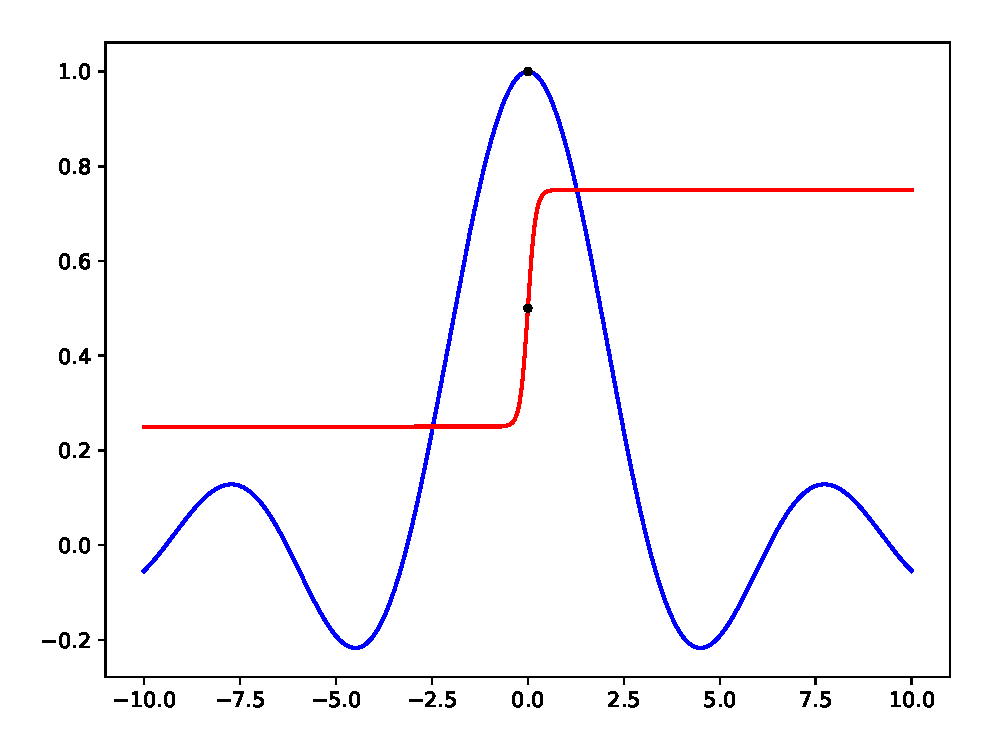
\includegraphics[]{./images/ex1}}

If \eqref{eq:grad-avg} were small for some set of indices
\(I\subseteq\{1,\dots,d\}\), we could freeze the associated variables to nominal
values \(\vx_{I}=\vx_{I,\text{Nom}}\). This would reduce the dimensionality of the
problem. Note that a purely local approach would \emph{not} endorse this
pick-and-freeze approach, as illustrated by the blue curve in Figure
\ref{fig:ex1}, repeated in the margin. Furthermore, this pseudoglobal approach
is prone to miss nonlinear behavior in the function -- imagine if we had sampled
outside the sharp region of the red curve in Figure \ref{fig:ex1}. A
pseudoglobal approach is not necessarily the best way to attack the problem of
freezing variables; this is better handled via global sensitivity analysis.

Determining the stability of an optimal point

Unconstrained optimization is conceptually straightforward; critical points are
found where the gradient of the qoi is zero. Optimal points are then found where
the curvature meets an additional criterion.\footnotemark The magnitude of the
curvature gives some sense of how sensitive the optimal point is to changes in
parameter values.

\footnotetext{e.g. for a maximum, we want negative curvature}

For constrained optimization, the intuition is slightly different. Rather than
having zero gradient, a function must meet a stationarity condition; its
gradient must `balance' that of the constraints.\footnote{More formally, the
Karush-Kuhn-Tucker (KKT) conditions give a set of first-order necessary
conditions for optimality.} Figure \ref{fig:opt} gives a cartoon example of a
constrained optimization problem. The punchline is that the gradient of our qoi
need not be zero for a constrained optimal point. This is not a big deal if our
parameters are known exactly.

\begin{figure}[!ht]
  \centering
  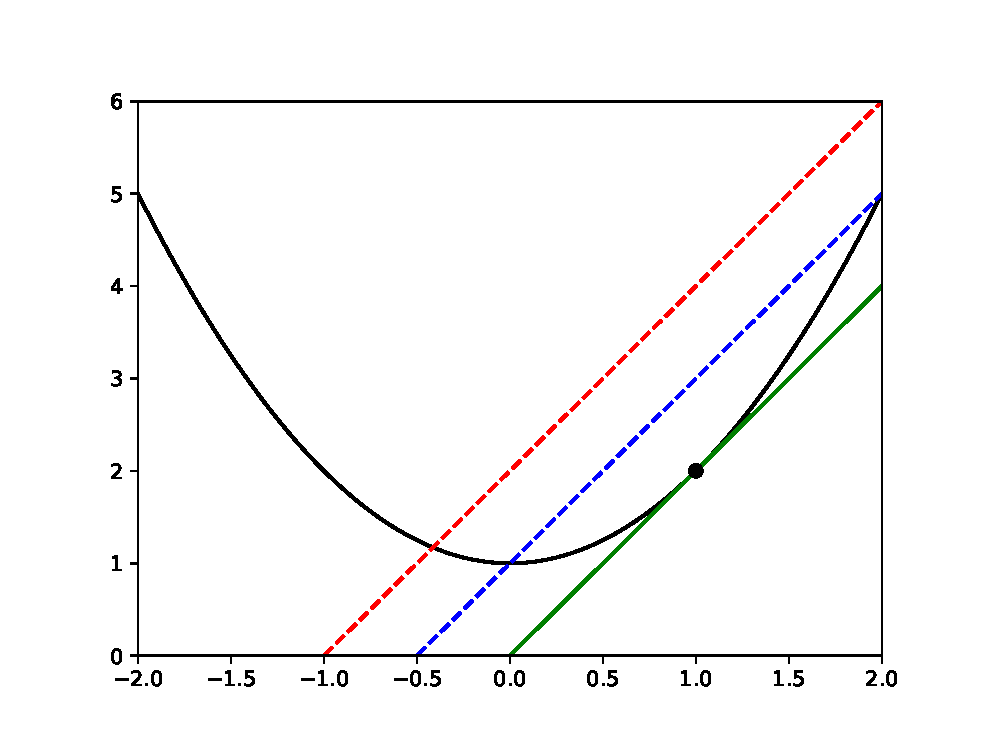
\includegraphics{./images/ex2}
  \caption{Cartoon of constrained optimization: The black curve is the
    constraint, while the red, blue, and green lines are isocontours of
    the qoi. If the gradient of our qoi is not aligned with the gradient
    of the constraint at their intersection -- if they are not \emph{tangent}
    -- then one can find an improved function value by sliding along the
    constraint. Here, the green isocontour is tangent at the black dot,
    which corresponds to an optimal point. The gradient of the qoi is
    nonzero at this point; if there is uncertainty in the input parameters,
    this could lead to the realized value of the response being significantly
    less than desired. One may quantify these effects through local sensitivity
    analysis}
  \label{fig:opt}
\end{figure}

However, if our parameters are uncertain, a nonzero gradient provides some
information about how much this uncertainty can affect our optimal value. As a
more concrete example in an engineering design context, one could do a Taylor
approximation to determine how much the qoi may fluctuate, then add margin to
the design to account for this uncertainty.

\subsection{Finite Differencing}
\label{sec:org90b543e}
Conceptually, approximating the derivative is quite simple. One simply chooses a
base point \(\vx\) and considers a finite step-size \(\Delta x\) approximation to
the derivative\footnote{Note that this is the \emph{partial derivative}, which is
usually denoted with \(\partial\). We're going to reserve the \(\partial\) symbol
for a different operation in these notes.}

\begin{equation}
  \frac{df}{dx_i} \approx \frac{f(x_1,\dots,x_i+\Delta x,\dots,x_d) - f(\vx)}{\Delta x}.
\end{equation}

However, there are some complications with this approach. First, this
computational procedure requires additional evaluations, with a cost that grows
linearly with dimensionality \(d\). If we require \(N\) evaluations of the gradient
for a desired procedure (e.g. building a map of the gradient or performing
quadrature), then our total cost will be \(O(Nd)\).

The other complication is choosing a sensible \(\Delta x\). Recent work has
studied the selection of \(\Delta x\) based on measuring the \emph{empirical noise} of
a function; that is, tailoring the step-size based on the observered variability
in a computed qoi arising from a computational procedure.\cite{more2012}

\subsection{Adjoint Method}
\label{sec:org39314ad}
The adjoint is clever method for cheaply computing the sensitivity of a scalar
qoi. This is particularly useful if evaluating our qoi requires solving some
parameterized governing equation \(F(\vy,\vx)\) for a state variable (e.g. flow
field) on which our qoi depends \(f(\vy,\vx)\). Practically, it allows us to
compute the total derivative of our qoi \(\frac{df}{d\vx}\) at the expense of one
additional solution comparable to \(F(\vy,\vx)\). Steven Johnson \cite{johnson2012}
has some very nice introductory notes on the topic, which I follow for the next
example. He also points to a paper by Cao et al.\cite{cao2003adjoint} which gives
a more general treatment of the adjoint.

Example: Linear System

The spirit of the adjoint method is well-illustrated by a simple linear system.
Suppose we have a governing equation for the state \(A_{jk}(\vx)y_k=b_j(\vx)\)
\footnote{I'm going to use \href{https://en.wikipedia.org/wiki/Einstein\_notation}{Einstein notation} here to help make this easier to
follow.}, where our equation is parameterized by \(\vx\). Our qoi is some known
function of the state and our parameters \(f(\vy,\vx)\). By chain rule, the
sensitivity is

\begin{equation}\label{eq:linear-sens}
\frac{df}{dx_i} = \frac{\partial f}{\partial x_i} %
+ \frac{\partial f}{\partial y_j}\frac{\partial y_j}{\partial x_i}.
\end{equation}

\noindent Since \(f\) is known, the partials \(\frac{\partial f}{\partial x_i}\) and
\(\frac{\partial f}{\partial y_j}\) are easy to evaluate.\footnote{Here, we use
\(\partial\) to denote a `direct' derivative. For example, if
\(f(\vx,\vy)=\sum_{i=j}^my_j\), then \(\frac{\partial f}{\partial x_i}=0\) and
\(\frac{\partial f}{\partial y_j}=1\).} However, the quantity \(\frac{\partial
y_j}{\partial x_i}\) is more challenging. Using the matrix inverse, we have
\(y_j=A_{jk}^{-1}b_k\). Taking the partial, we have\footnotemark

\footnotetext{Here, we use the identity $\frac{\partial \mA^{-1}}{\partial s} =-\nobreak
\mA^{-1}\frac{\partial \mA}{\partial s}\mA^{-1}$. One can derive this by
re-arranging $\frac{\partial(\mA^{-1}\mA)}{\partial s}$.}

\begin{equation}\begin{aligned}
\frac{\partial y_j}{\partial x_i} &= \frac{\partial A^{-1}_{jk}}{\partial x_i}b_k + A^{-1}_{jk}\frac{\partial b_k}{\partial x_i}, \\
&= A^{-1}_{jk}\left(-\frac{\partial A_{kl}}{\partial x_i}A^{-1}_{lp}b_p+\frac{\partial b_k}{\partial x_i}\right), \\
&= A^{-1}_{jk}\left(-\frac{\partial A_{kl}}{\partial x_i}x_l+\frac{\partial b_k}{\partial x_i}\right).
\end{aligned}\end{equation}

\marginnote{Using Einstein notation makes it clear in \eqref{eq:linear-sens2}
that the quantity $\frac{\partial A_{kl}}{\partial x_i}$ is a rank 3 tensor, as
there are three indices.}

\noindent Substituting into \eqref{eq:linear-sens} yields

\begin{equation}\label{eq:linear-sens2}
\frac{df}{dx_i} = \frac{\partial f}{\partial x_i} + \frac{\partial f}{\partial y_j}A^{-1}_{jk}%
\left(-\frac{\partial A_{kl}}{\partial x_i}y_l + \frac{\partial b_k}{\partial x_i}\right).
\end{equation}

One could evaluate \eqref{eq:linear-sens2} by carrying out the matrix
multiplication (which would be expensive), or by carrying out the product
\(\frac{\partial f}{\partial y_j}A^{-1}_{jk}\equiv\nobreak\lambda_k\). This
quantity is the solution of the \emph{adjoint equation}

\begin{equation}\label{eq:linear-adjoint}
\lambda_k A_{kj} = \frac{\partial f}{\partial y_j}.
\end{equation}

In summary, to compute the sensitivity via the adjoint method, we need (1) the
solution to the governing equation \(\vy\) at our chosen parameter values, (2) the
partial derivatives to known functions \(\frac{\partial f}{\partial x_i},
\frac{\partial f}{\partial y_j}, \frac{\partial A_{kl}}{\partial x_i},
\frac{\partial b_k}{\partial x_i}\), and (3) the solution to the adjoint equation
\(\lambda_k\). We then evaluate the total derivative via

\begin{equation}
\frac{df}{dx_i} = \frac{\partial f}{\partial x_i} + \lambda_k A^{-1}_{jk}\left(-\frac{\partial A_{kl}}{\partial x_i}y_l + \frac{\partial b_k}{\partial x_i}\right).
\end{equation}

\subsection{Conclusion}
\label{sec:org9f00d47}
This set of notes introduced the motivation behind sensitivity analysis, the
broad philosophies of local and global approaches, some uses of sensitivity
analysis, and approaches for performing local sensitivity analysis. Next time,
we'll dig into techniques for performing global sensitivity analysis.

\subsection{Appendix}
\label{sec:org880d431}
\subsection{Some useful derivations}
\label{sec:org1df2b75}
Personally, I found some of the claims in Johnson's notes rather
mysterious.\cite{johnson2012} I attempt to demystify some of those points in this
section.

The derivative of a matrix exponential ends up being a convolution. This is
because the derivative is more easily carried out in the frequency domain, and
we pick up a convolution from doing so. Let \(\mA=\exp(-t\mB)\). First,
we'll work out the Laplace transform of this quantity.

\begin{equation}
  \cL\{\mA\}(s) = (s\mI+\mB)^{-1}.
\end{equation}

\noindent Next, we'll take the derivative, using the identify
\(\frac{\partial\mA^{-1}}{\partial
x}=\nobreak-\mA^{-1}\frac{\partial\mA}{\partial x}\mA^{-1}\).

\begin{equation}
  \frac{\partial}{\partial x}\cL\{\mA\}(s) = %
    -(s\mI+\mB)^{-1}\frac{\partial\mB}{\partial x}(s\mI+\mB)^{-1}.
\end{equation}

\noindent Finally, we'll take an inverse Laplace transform,\footnote{Assuming we can
commute the derivative with the integral} which yields

\begin{equation}\begin{aligned}
  \frac{\partial\mA}{\partial x} &= -\left[e^{-\mB t}\frac{\partial\mB}{\partial x}\right] %
    \circledast \left[e^{-\mB t}\right], \\
    &= -\int_0^t e^{-\mB t'}\frac{\partial\mB}{\partial x}e^{-\mB(t-t')}dt'
\end{aligned}\end{equation}

This enters into the derivative equation via

\begin{equation}\label{eq:adj-time}
  \frac{df}{dx_i}(t) = \frac{\partial f}{\partial x_i}(t) + \lambda_k(t)%
    \left(-\frac{\partial A_{kl}}{\partial x_i}(t) y_l(t) + \frac{\partial y_k}{\partial x_i}(0)\right).
\end{equation}

In Johnson's notes, he states a form equivalent to

\begin{equation}\label{eq:shifted}
  \frac{df}{dx_i}(t) = \frac{\partial f}{\partial x_i}(t) + %
    \int_0^t\lambda_k(t-t')\frac{\partial\mB}{\partial x_i}y_l(t')dt' + %
    \lambda_k(t)\frac{\partial y_k}{\partial x_i}(0).
\end{equation}

This varies from what one might expect as the `plug in' result from manipulating
\eqref{eq:adj-time}. However, recall that the matrix exponential acts as a shift
operator -- it \emph{shifts} initial data forward (or backward) in time to give the
solution at a desired time. Commuting terms and applying the shifts results in
\eqref{eq:shifted} above.

\subsection{Global Sensitivity Analysis}
\label{sec:org81b0ac8}
Last time, we talked about local sensitivity analysis, both in terms of how we
might use the derivative, and how we might go about computing it. While useful
for various purposes, local sensitivity fails to capture trends outside a
selected neighborhood. This is what global sensitivity seeks to address. Figure
\ref{fig:ex1} illustrates problematic behavior for both local and global
approaches.

\begin{figure}[!ht]
  \centering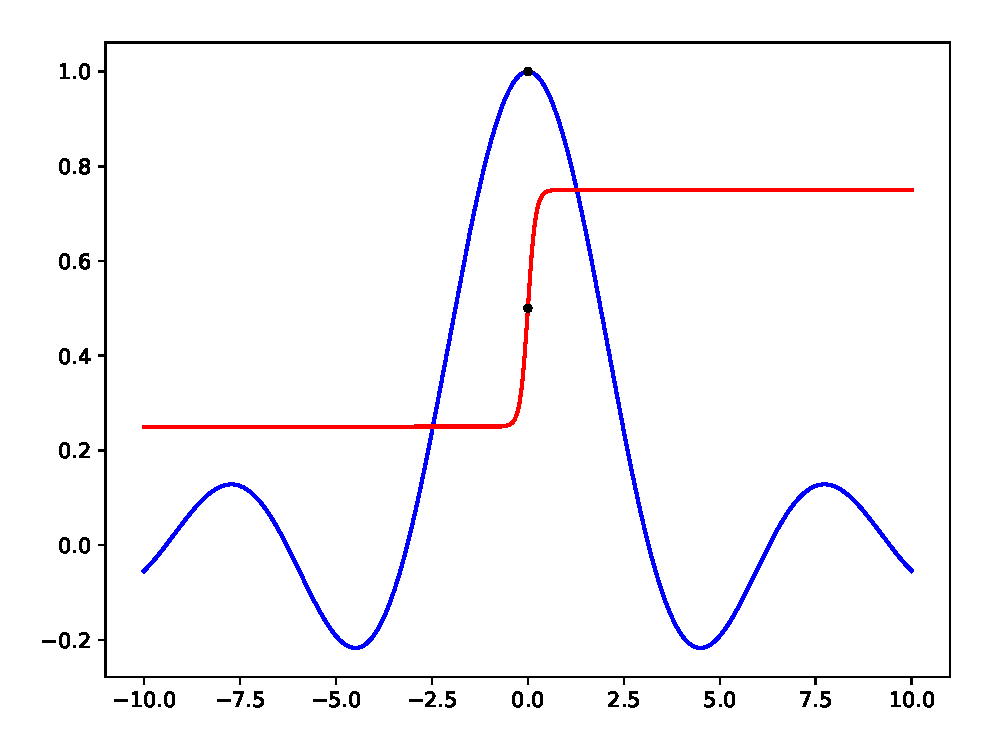
\includegraphics[width=0.75\textwidth]{./images/ex1}
  \caption{Local sensitivity would fail to capture the behavior of the blue
  function (in terms of giving zero sensitivity) at the point of interest (black dot),
  whereas global sensitivity would return a finite value.}
  \label{fig:ex1}
\end{figure}

Dimension reduction

Why perform global sensitivity analysis? One reason is to perform \emph{dimension
reduction}; that is, principled reduction of the dimensionality of a system.
Figure \ref{fig:curse} depicts the \emph{curse of dimensionality}, which states
(roughly) that the computational expense of a procedure tends to grow
\emph{exponentially} with the dimension of the problem. The most direct way to
address this issue is to reduce dimensionality -- to reduce the number of input
parameters we need to consider.

Suppose we perform a sensitivity analysis and find that our qoi \(f(\vx)\) is
relatively unaffected by its input \(x_1\). We could set \(x_1=c\) to a constant
nominal value, and continue with \(f(c,x_2,\dots,x_d)\), which has dimension
\(d-1\). This would reduce the expense involved with studying our qoi, and since
the reduction is \emph{exponential} this could potentially enable studies previous
intractable. Global sensitivity analysis provides principled tools to perform
dimension reduction.

\begin{figure}[!ht]
  \centering
  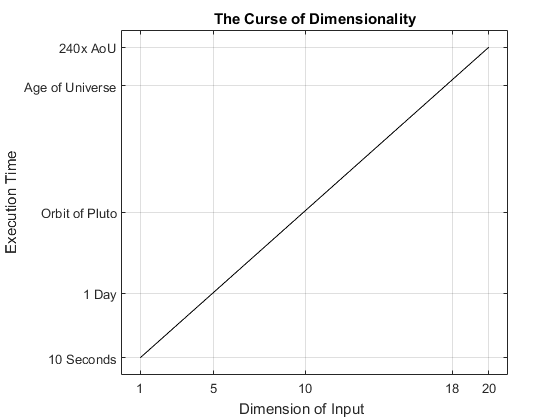
\includegraphics[width=0.75\textwidth]{./images/curse_of_dimensionality}
  \caption{Cartoon depicting computational expense under the Curse of Dimensionality.
  The most direct way to address this curse is to reduce the effective dimension
  of our problem. One way to reduce dimensionality is to identify parameters
  which are unimportant, and freeze them to nominal values. Global sensitivity
  analysis allows us to determine such unimportant factors.}
  \label{fig:curse}
\end{figure}

We'll study three types of global sensitivity analysis:
\begin{enumerate}
\item Morris Screening, which seeks to identify unimportant parameters in an economical fashion.
\item Active Subspaces, which identify important \emph{directions} in parameter space.
\item Sobol Indices, which attribute variability in the output to particular parameters.
\end{enumerate}

Parameter interactions

So far in sensitivity analysis, we have only talked about derivatives. For the
first derivative, we consider the change in a function as we perturb a single
variable. In the case where parameters only affect our qoi linearly, this is
sufficient, as effects are additive. However, if there are nonlinear
\emph{interactions} between parameters, this presents an issue for this one-at-a-time
style of sensitivity analysis. As a concrete example, consider the function

\begin{equation}
  f = 0.3 x_1 + 8.0 x_1 x_2,
\end{equation}

\noindent on the domain \(\vx\in[0,1]^2\). Clearly, the mixed term dominates the
behavior of the function. The first derivative does not capture this interactive
effect, by definition. Capturing interactions of parameters could be
accomplished by considering the second derivative, as is done in generalizations
of Morris screening. However, the Sobol indices handle this by a different means
entirely.

\subsection{Morris Screening}
\label{sec:orgf5d704d}
Morris screening is closely related to the derivative, and can be thought of as
studying the mean and variance of the derivative. The textbook
\cite{smith2013uncertainty} goes through this procedure in gory detail; these
notes will give only a brief introduction, as we'll focus more on Sobol indices.
Morris screening considers statistics of the \emph{elementary effects}, defined by

\begin{equation}\label{eq:elem-effect}
  d_{i}(\vx_j) = \frac{f(\vx_j+\Delta \ve_i) - f(\vx_j)}{\Delta},
\end{equation}

\noindent where \(\ve_i\) is the i-th standard basis vector,\footnote{The vector with
all zeros, except for a one in the i-th entry} and \(\Delta\) is a large stepsize.
Note that \eqref{eq:elem-effect} is simply a first-order approximation of the
derivative; however, since \(\Delta\) is relatively large, this is a coarse
approximation to the derivative. These elementary effects are used to construct
global sensitivity measures

\begin{equation}\begin{aligned}
  \mu_i^* &= \frac{1}{r}\sum_{j=1}^r |d_{i}(\vx_j)|, \\
  \sigma_i^2 &= \frac{1}{r-1}\sum_{j=1}^r(d_{i}(\vx_j)-\mu_i)^2, \mu_i=\frac{1}{r}\sum_{j=1}^rd_{i}(\vx_).
\end{aligned}\end{equation}

Note that considering elementary effects misses interactions, for the reasons
discussed above. Generalizations of this technique consider higher-order
derivatives, which probe interactions. This procedure is called \emph{screening}
because it allows us to determine whether individual parameters are unimportant,
but does not quantify relative variable importance. To determine relative
importance, we can turn to Sobol indices. However, Morris screening is a
relatively cheap procedure, and thus is a good tool to be aware of.

\subsection{Active Subspaces}
\label{sec:org7724f8f}
The active subspace is a more recent dimension reduction technique, and is
somewhat different in spirit from other global sensitivity analysis
procedures.\cite{constantine2015} Consider the function

\begin{equation}\label{eq:as-ex}
  f(\vx) = \f12(0.3x_1+0.7x_2)^2.
\end{equation}

\noindent For this qoi, both its parameters are important. However, the function
clearly varies only along the direction \((0.3,0.7)^T\), and not at all along the
direction \((0.7,-0.3)^T\). Rather than picking and freezing individual
parameters, the active subspace considers \emph{linear combinations} of the inputs
which are important. These correspond to directions in parameter space. Figure
\ref{fig:as-ex} depicts the active subspace for \eqref{eq:as-ex}.

\begin{figure}[!ht]
  \centering
  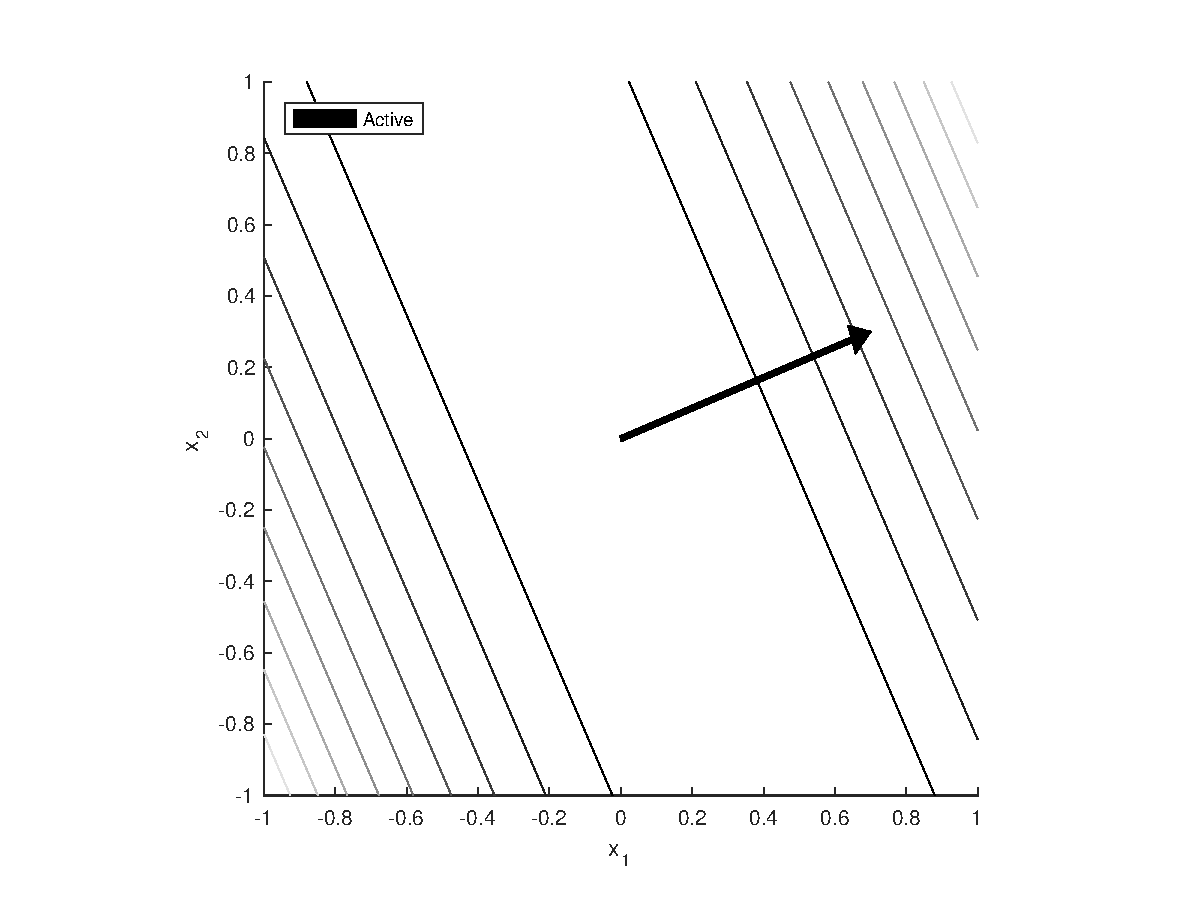
\includegraphics[width=0.75\textwidth]{./images/contour_plot}
  \caption{Isolines and active direction for \eqref{eq:as-ex}}
  \label{fig:as-ex}
\end{figure}

The active subspace is computed by studying the outer product of the gradient;
taking an expectation with respect to the density for \(\vx\), we define

\begin{equation}\label{eq:as-c}
  \mC = \E[\nabla_{\vx}f\nabla_{\vx}f^T].
\end{equation}

\noindent Note that \(\mC\) is symmetric semi-positive definite, thus it admits an
eigenvalue decomposition \(\mC=\mW\m\Lambda\mW^T\). A basis for the active
subspace is identified by separating the magnitude-ordered eigenvalues
\(\m\Lambda=\text{Diag}([\m\Lambda_a,\m\Lambda_i])\) and their associated
eigenvectors \(\mW=[\mW_a,\mW_i]\). This split is often chosen based on the
relative magnitude of the eigenvalues.

In contrast with Morris screening, we may use the eigenvalues \(\lambda_i\) to
rank the associated directions \(\vw_i\). The \(\lambda_i\) are related to the
mean-squared directional derivative associated with the appropriate eigenvector.
Thus, ranking the directions can only be done in an average sense; the
eigenvalues may hide extreme local behavior. Furthermore, the active subspace
requires gradient information; this is fine if we access to this information,
say through an adjoint solver. If gradients are unavailable, we would need to
turn to other approaches, such as finite differences or surrogate modeling,
which increases the expense.

Exploiting the active subspace involves a number of challenges, and is both
application dependent and an active area of research. To illustrate some of
these challenges, suppose we define the \emph{active} and \emph{inactive variables} based
on the decomposition above

\begin{equation}\begin{aligned}
  \vx_a &= \mW^T_a\vx, \\
  \vx_i &= \mW^T_i\vx.
\end{aligned}\end{equation}

\noindent We would like to re-parameterize our qoi in terms of the \(\vx_a\) to
reduce dimensionality. However, the naive statement \(f(\vx)=f(\mW_a\vx_a)\) is
false! Furthermore, we must determine the domain of \(\vx_a\); this is a
projection of the original domain \(\Omega\) on the subspace \(\cR(\mW_a)\), which
is in general quite complicated.

\subsection{Sobol Indices}
\label{sec:orgd776a4d}
Both Morris screening and the active subspace consider some average of the
gradient. In contrast, Sobol indices are based on \emph{variance}. The Sobol indices
may be used to attribute variance of the qoi to subsets of the input parameters.
It is a useful, well-studied, and commonly-used technique for global sensitivity
analysis, so we will spend some time discussing it.

Sobol indices require a random variable interpretation of our quantity of
interest, so we'll introduce some notation used throughout the section. Let
\(\mX\sim\rho\) be our random input parameters, distributed according to a joint
density \(\rho\) over our parameter space \(\Omega\).\footnote{Sobol indices also have
some properties that rely on \emph{independence} of the input parameters. We will
return to this point later.} Then our output qoi is also a random variable
\(Y=f(\mX)\). We denote by \(\E[Y] = \int f(\vx)\rho(\vx)d\vx\) the expectation, and
by \(\V[Y]=\E[(Y-\E[Y])^2]\) the variance. Note that the following useful identity
involving the variance holds

\begin{equation}
  \V[Y] = \E[Y^2] - \E[Y]^2.
\end{equation}

We denote conditioning by a vertical bar; this corresponds to holding particular
random inputs fixed in value, and leaving them out of the integral for a
particular expectation. For example, if \(Y=f(X_1,X_2,X_3)\), then

\begin{equation}
  \E_{X_2,X_3}[Y|X_1=x_1] = \int f(x_1,x_2,x_3)\rho(x_1,x_2,x_3)dx_2dx_2,
\end{equation}

\noindent where we use subscripts to make explicit the integration variables.
Note that \(\E_{X_2,X_3}[Y|X_1]\) is still a random variable\footnote{when it lacks the
equality \(X_1=x_1\)}, due to the variability arising from \(X_1\). We will use
conditional variance to decompose the total variance \(\V[Y]\) according to
different input contributions. This will involve expressions of the sort
\(\E_{X_2,X_2}[\V_{X_1}[Y|X_1]]\).\footnote{which is no longer a random variable, as we
have integrated out all of the parameters}

In what follows, we will drop the variable subscripts, as they tend to render
expressions indecipherable. The same information is implied by the conditioning;
the expression \(\V[Y|X_1]\) carries out the integration keeping \(X_1\) fixed,
which is then integrated out in the expression \(\E[\V[Y|X_1]]\).

Intuition

The Sobol indices are based on a decomposition of the variance of our output
qoi.\footnote{This necessitates a random variable interpretation of both our inputs
and outputs. In the absence of `truly' random inputs, one can assign uniform
distributions to the uncertain parameters.} In the next section, we'll look at a
formal treatment using the functional analysis of variance. Before that, we'll
go through a more simple treatment of the same problem, in order to build
intuition.\footnote{The primer by Saltelli et al.\cite{saltelli2004sensitivity} is a
good, quick read on sensitivity analysis. I follow that text for this
subsection.}

First, we will introduce some notation to help keep track of variable subsets.
Let \(\vu\) be an \emph{index set}; that is \(\vu\subseteq\{1,\dots,d\}\). We will use
\(\vu\) to denote subsets of the input variables; in the example above, we used
\(\vu=\{2,3\}\) to give us \(\mX_{\vu}=\{X_2,X_3\}\). Let \(-\vu\) be the set
complementary to \(\vu\) with respect to \(\{1,\dots,d\}\); in the example above
\(-\vu=\{1\}\).

Next, we will prove a simple identity, which will allow us to attribute the
variance \(\V[Y]\) to different inputs. Note that for any index set \(\vu\), we have

\begin{equation}\begin{aligned}\label{eq:var-decomp}
  \E[\V[Y|\mX_{\vu}]] + \V[\E[Y|\mX_{\vu}]] &= %
  \E[\E[Y^2|\mX_{\vu}] - \cancel{ \E[Y|\mX_{\vu}]^2 }] \\
  &+ \cancel{\E[\E[Y|\mX_{\vu}]^2]} - \E[\E[Y|\mX_{\vu}]]^2, \\
  &= \E[Y^2] - \E[Y]^2, \\
  &= \V[Y^2].
\end{aligned}\end{equation}

\noindent \Cref{eq:var-decomp} allows us to decompose the variance into two
terms \emph{that we can interpret}. First, note that the expression
\(\V[\E[Y|X_{\vu}]]\) first averages out all the variables \(\mX_{-\vu}\), then
computes the variance due only to \(\mX_{\vu}\). We may use this expression with a
singleton index set \(\vu=\{i\}\) to define the \emph{first-order sensitivity index}

\begin{equation}\label{eq:sobol-first}
  \underline{\tau}_{\{i\}}^2 = \frac{\V[\E[Y|X_i]]}{\V[Y]}.
\end{equation}

\noindent \Cref{eq:sobol-first} is bounded between \([0,1]\), and enables us to
rank variables according to their importance. Practically
\(\underline{\tau}_{\{i\}}^2\) tells us how much variance reduction we could
expect if we were able to exactly freeze \(\mX_i\). We could use this information
to inform which variables we should better characterize, in order to reduce
variability.

Note that we should \emph{not} use \(\underline{\tau}_{\{i\}}^2\) to perform dimension
reduction; the first-order index does not account for interactions with other
variables, so we may miss some important cross terms. Instead, we may consider
the \emph{total-order sensitivity index}

\begin{equation}\label{eq:sobol-total}
  \overline{\tau}_{\{i\}}^2 = \frac{\E[\V[Y|X_{-\{i\}}]]}{\V[Y]} = %
  1 - \frac{\V[\E[Y|X_{-\{i\}}]]}{\V[Y]}.
\end{equation}

\noindent \Cref{eq:sobol-total} is also bounded between \([0,1]\), and accounts
for interactions between \(X_i\) and all other variables. We may interpret
\eqref{eq:sobol-total} in at least two ways: As the variability in \(Y\) due to
\(X_i\), averaged over all other inputs (middle expression), or as the complement
of the variability arising from all the variables excluding \(X_i\) (right
expression). If \(\overline{\tau}_{\{i\}}^2\) is zero or small, we can be
confident that \(X_i\) contributes little to the variablility in \(Y\), neither
through first-order nor interaction effects.

In summary: The notation for the sensitivity indices is suggestive of their use.
The first-order index \(\underline{\tau}_{\{i\}}^2\) can be thought of as a
\emph{lower} bound; if it is large, then we can be confident that \(X_i\) is
\emph{important}. In contrast the total-order index \(\overline{\tau}_{\{i\}}^2\) is an
\emph{upper} bound; if it is small, then we can be confident that \(X_i\) is
\emph{unimportant}.

The next section gives a more formal treatment of Sobol indices coming from the
functional ANOVA decomposition. It's optional reading.

Formulation

Sobol indices are based on the functional analysis of variance (ANOVA)
decomposition.\footnote{For those with a statistics background, the functional ANOVA
is a generalization of the multiple-way ANOVA to functions of multiple
variables.} The textbook considers only first- and second-order terms; to
provide some additional details, we'll follow the notation of Owen
\cite{owen2013variance} and consider all higher-order terms.

We start by assuming the input parameters are statistically independent, and
uniform on \(\vx\in[0,1]^d\).\footnote{If the parameters are independent and
well-behaved, we can map them to a uniform distribution. The assumption of
independence is a common, but rather strong assumption. More on this later.} The
functional ANOVA decomposition is given by

\begin{equation}\label{eq:f-anova}
  f(\vx) = \sum_{u\subseteq\cD} f_u(\vx),
\end{equation}

\noindent where \(u=\{j_1,\dots,j_{|u|}\}\) is an index set, \(|u|\) denotes
cardinality,\footnote{The number of elements in a set.} and the \(f_u\) are defined
recursively by

\begin{equation}\begin{aligned}\label{eq:f-anova-rec}
  f_u(\vx) &= \int\left(f(\vx)-\sum_{v\subset u} f_v(\vx)\right)d\vx_{-u}, \\
  &= \int f(\vx)d\vx_{-u} - \sum_{v\subset u} f_v(\vx),
\end{aligned}\end{equation}

\noindent where \(\{v\subset u\}\) denotes all proper subsets \(v\) of \(u\), and
\(-u=u^c\) is the complementary set. To unpack this statement, first note that
\(f_{\varnothing}=\int f(\vx)d\vx=\mu\) is simply the mean of the function. The
singletons \(f_{\{i\}}\) are called the \emph{main effects}; these retain variability
in a single parameter. For example, for \(i=1\) we have

\begin{equation}
  f_{\{1\}}(x_1) = \int f(x_1,x_2,\dots,x_d)dx_2\cdots dx_d - f_{\varnothing}.
\end{equation}

\noindent The functions \(f_u\) with \(|u|>1\) describe the \emph{interactions} in
isolation of the main effects, which are subtracted off. In this way, each \(f_u\)
considers a separate component of the variability.

The variance of the qoi is given by \(\sigma^2=\int(f(\vx)-\mu)^2d\vx\), and the
ANOVA identity allows us to sum the separate contributions via

\begin{equation}\label{eq:anova-idet}
  \sigma^2 = \sum_u \sigma_u^2,
\end{equation}

\noindent where \(\sigma_u^2 = \int f_u(\vx)^2d\vx\) for \(u\neq\varnothing\), and
\(\sigma_{\varnothing}^2=0\). \Cref{eq:anova-idet} is extremely useful, and
enables us to apportion fractions of the variance to different combinations of
the input parameters.

Sobol \cite{sobol1993} introduced two sensitivity indices, defined by

\begin{equation}\begin{aligned}\label{eq:sobol-indices}
  \underline{\tau}_u^2 = &\sum_{v\subseteq u}\sigma_v^2, \\
  \overline{\tau}_u^2 = &\sum_{v\cap u\neq\varnothing}\sigma_v^2. \\
\end{aligned}\end{equation}

\noindent The index \(\underline{\tau}_u^2\) is called the \emph{closed} sensitivity
index, while \(\overline{\tau}_u^2\) is called the \emph{total} sensitivity index. In
words, the closed index considers the set of parameters \(u\) and all its subsets.
The total index considers \(u\), and any component which involves this subset in
any way. One can show that \(\underline{\tau}_u^2\leq\overline{\tau}_u^2\), which
is intuitive given the definition. These indices are usually studied in
normalized form \(\underline{\tau}_u^2/\sigma^2\) and
\(\overline{\tau}_u^2/\sigma^2\), which in light of \eqref{eq:anova-idet} can be
interpreted as fractions of the total variance.

These two indices are used in different ways. If the total index
\(\overline{\tau}_u^2\) is small, it conclusively shows that the entire subset of
variables \(u\) is unimportant. If the closed index \(\underline{\tau}_u^2\) is
large, it conclusively shows the set of variables \(u\) cannot be neglected.

Computation

The Sobol indices are defined via \emph{expectations} \(\E[Y]=\E[f(\mX)]=\int
f(\vx)\rho(\vx)d\vx\); integrals of a quantity against the random variable
density. Evaluating these expressions directly requires evaluating a
multi-dimensional integral; however, integration is subject to the curse of
dimensionality! We started looking at sensitivity analysis to avoid this curse,
so we need a different way.

A simple way to approximate an expectation is via the \emph{Monte Carlo} method; this
involves drawing independent samples from the distribution \(\vx_i\sim\rho\) for
\(i=1,\dots,n\), and constructing the sample estimate

\begin{equation}
  \E[f(\mX)] \approx \frac{1}{n}\sum_{i=1}^n f(\vx_i).
\end{equation}

Naive estimation of the Sobol indices via Monte Carlo can be expensive, as they
involve \emph{nested expectations} for a cost of \(O(n^2)\). Sobol \cite{sobol1993}
introduced a trick for a less expensive (\(O(2n)\))\footnote{Yes, this is formally
\(O(n)\); I'm just emphasizing the fact that we need to evaluate two points for
each sample when using the hybrid point method.} estimate using \emph{hybrid} points.
These hybrid points are denoted by \(\vy=\vx_u:\vz_{-u}\), where \(y_j=x_j\) for
\(j\in u\), and \(y_j=z_j\) for \(j\not\in u\). We sample \(n\) pairs
\(\vx_i,\vz_i\overset{\text{iid}}{\sim} U(0,1)^d\), and approximate

\begin{equation}\begin{aligned}
  \hat{\mu} &= \frac{1}{2n}\sum_{i=1}^n(f(\vx_i)+f(\vx_{i,u}:\vz_{i,-u})), \\
  \hat{\underline{\tau}}_u^2 &= \frac{1}{n}\sum_{i=1}^n f(\vx_i)f(\vx_{i,u}:\vz_{i,-u})-\hat{\mu}^2, \\
  \hat{\overline{\tau}}_u^2 &= \frac{1}{n}\sum_{i=1}^n(f(\vx_i)-f(\vx_{i,-u}:\vz_{i,u}))^2.
\end{aligned}\end{equation}

Stochastic codes

Note that in Monte Carlo, we draw samples \emph{randomly}, and average them to form
our estimate. This implies that our results are themselves random. Unlike a
deterministic code, which will return the same output for the same input, simply
re-running a stochastic code with the same input will produce variable outputs;
a single output of a stochastic process is called a \emph{realization}. Making
statements about a random process based on a single realization is like rolling
a die a single time, and using that single number to make statements about the
entire random process. Thus, when studying the behavior of a stochastic code, it
is not appropriate to study a single realization alone.

As a concrete example, the quantity \(\hat{\mu}\) above is a sample estimate of
the quantity \(\E[f(\vx)]\); we call \(\hat{\mu}\) a \emph{point estimate}. By itself, a
point estimate gives no notion of how variable our estimate is. To that end, it
is standard practice to construct a \emph{confidence interval} (CI) separate from our
point estimate. A confidence interval is constructed at a desired \emph{confidence
level} (e.g. \(95\%\) confidence), and provides a quantitative notion of
variability. If our CI is very wide, it demonstrates a large uncertainty about
our estimate; conversely, if our CI is very narrow, we are fairly certain about
our estimate.\footnote{Note that formally, the confidence we have in these approaches
is in the \emph{procedures}, and not the \emph{results} themselves. A \emph{method} for
constructing a confidence interval has a particular confidence level. An
\emph{interval} itself either contains the true value or does not.}

One easy way to construct an \emph{approximate}\footnote{The precise definition of a
confidence interval is framed in terms of \emph{probabilistic coverage}. An
exact CI contains the true value being estimated with probability equal to the
confidence level. An approximate interval may be biased, or have a different
coverage probability, but should be constructed such that it asymptotically
(\(n\to\infty\)) recovers the exact interval.} confidence interval is to make a
\emph{normal approximation}. For this, we assume our quantity \(f(\vx)\sim
N(\mu,\sigma^2)\) is distributed according to an unknown normal distribution. If
this assumption were true, then we would have

\begin{equation}\label{eq:est-dist}
  \frac{1}{n}\sum_{i=1}^n f(\vx_i) \sim N(\mu,\sigma^2/n).
\end{equation}

\noindent If we knew \(\sigma^2\) exactly, we could easily construct a \(95\%\)
confidence interval about our point estimate via
\([\hat{\mu}-1.96\sigma/\sqrt{n},\hat{\mu}+1.96\sigma/\sqrt{n}]\).\footnote{The value
\(1.96\) is the approximate value of the \(97.5\%\) point of the standard normal
distribution; it effectively cuts off \(2.5\%\) on the right tail. Since we
construct the interval symmetrically about the estimate, this adds up to \(5\%\)
in the tails to capture the desired \(95\%\) confidence.} Note that the size of
the interval shrinks at a rate \(1/\sqrt{n}\); it is for this reason that Monte
Carlo is said to exhibit ``square-root convergence''.

If \(n\) is large, we would be justified in using the `plug-in principle' --
taking the variance estimate \(s^2=\frac{1}{n-1}\sum_{i=1}^n(f(\vx)-\hat{\mu})^2\)
and substituting it for \(\sigma^2\). However if \(n\) is small, this will not be a
good approximation. Furthermore, the normal assumption may be quite poor,
depending on \(f\) and the true distribution of \(\vx\); if we assume
\(\hat{\overline{\tau}}_u^2\) is normally distributed, this introduces the
possibility of the index taking a negative value. This is clearly impossible for
the true \(\overline{\tau}_u^2\), and CI constructed under the normal assumption
at low sample counts could give unrealistic results.

The normal approximation is endorsed by the \emph{central limit theorem}, which
(roughly) states that the sum of \(n\) independent, identically distributed random
variables tends towards a normal distribution as \(n\to\infty\).\footnote{With some
additional requirements; the iid random variables must have finite mean and
variance as well.} For large sample sizes \(n\), both \(\hat{\mu}\) and \(s^2\) will
be very nearly normal, endorsing the simple CI procedure above.

As a final note, when studying a simple problem for verification purposes, one
can always re-run the procedure to build an ensemble of results.\footnote{One might
be tempted to iterate the random seed while re-running the code. This can create
some subtle issues. For more notes on numerical paranoia, see Chapter 3 of Art
Owen's book on Monte Carlo.\cite{owen2013montecarlo}} We could compute the
variance based on the approximately-normal \(\hat{\mu}\) estimates, and construct
confidence intervals based on this quantity. However, since we are not re-using
samples, but instead drawing new ones for each estimate, this is a more
accurate, albeit more expensive, procedure.

Correlated parameters

The requirement of independent parameters is quite limiting, as many practical
problems of interest exhibit correlations between inputs. There exist other
sensitivities which overcome these concptual issues; for example, Shapley
values. \cite{owen2017shapley} However, computational issues involved with
correlated parameters still remain -- this is considered a hard problem, and is
an active area of research.

\end{document}
